\chapter{Experiment: Separation of two sources using partial decay rate
\label{chap:decaysep}}

% plot produced with
% plot_pep_3_3d.py
\begin{figure}[!t]
    \centering
    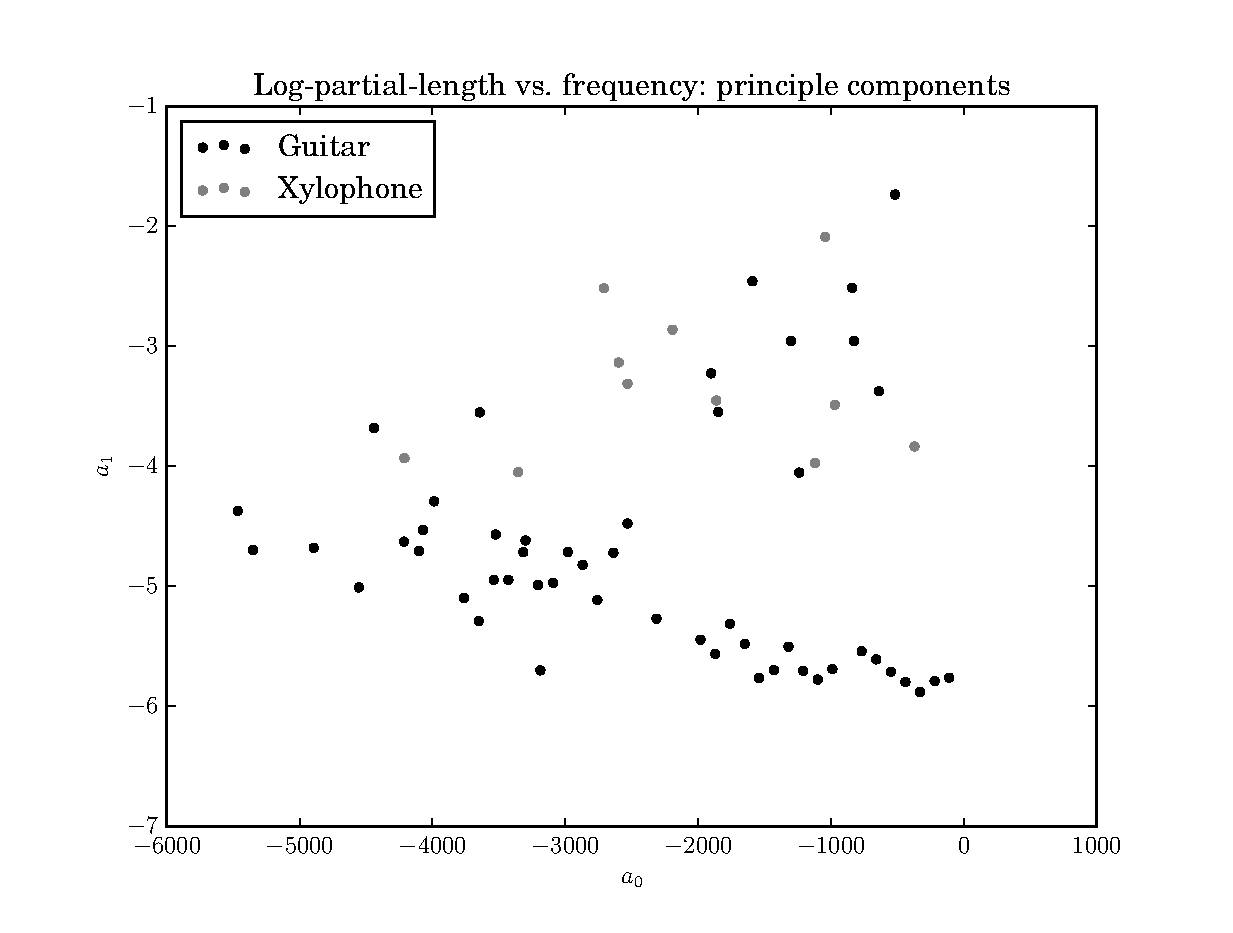
\includegraphics[width=\figwidthscale\textwidth]{plots/partial_classification_acgtr_xylo_sep_true_memberships.eps}
    \CaptionWithTitle{%
        \input{plots/partial_classification_acgtr_xylo_sep_true_memberships.txt}%
    }{This shows the distribution of partials when plotting their two principal components
        derived from their mean frequency and log-length. In this case, the
        source memberships of the partials are known. We see that there is
        generally a separation of the partials into two clusters corresponding
        to the two sources.
        \label{plot:partialclassificationacgtrxyloseptruememberships}}
\end{figure}

% plots produced with ../../signal_modeling/test/partial_estimation_plot_3_3c.py
\begin{figure}[!t]
    \centering
    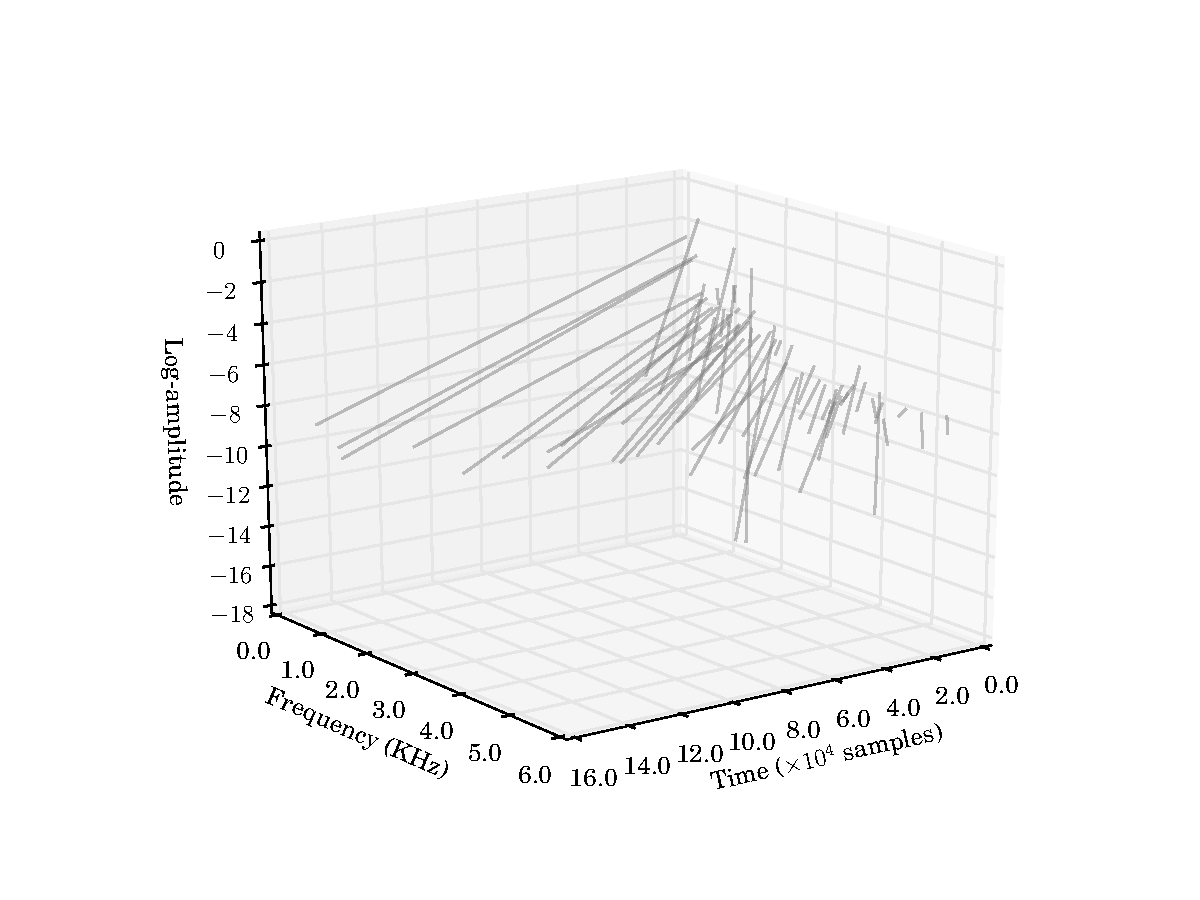
\includegraphics[width=\figwidthscale\textwidth]{plots/partial_classification_acgtr_xylo_partial_trajectories.pdf}
    \CaptionWithTitle{%
        \input{plots/partial_classification_acgtr_xylo_partial_trajectories.txt}%
    }{\label{plot:parclassaxpartialtrajectories}}
\end{figure}

\begin{figure}[!t]
    \centering
    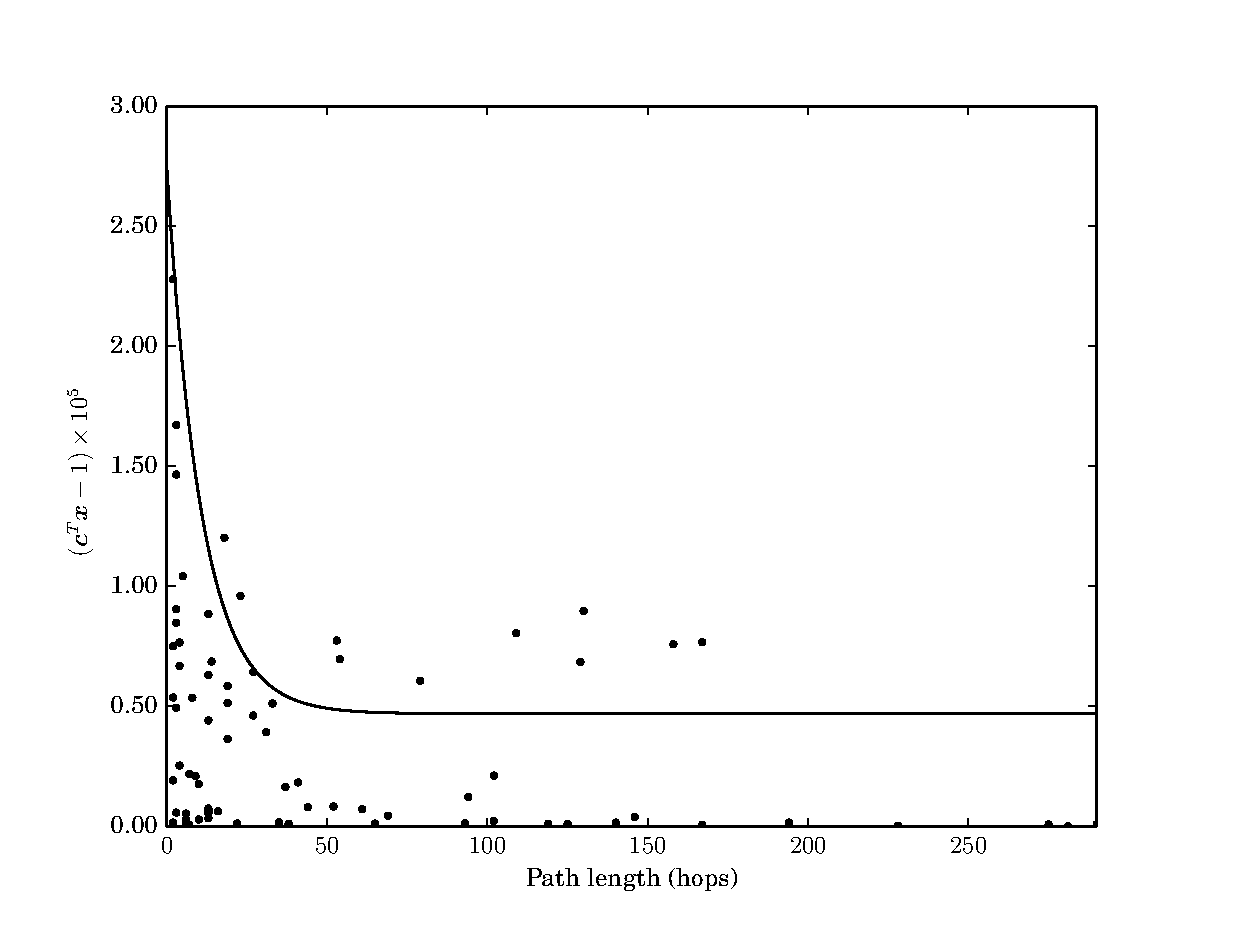
\includegraphics[width=\figwidthscale\textwidth]{plots/partial_estimation_acgtr_xylo_pcost_vs_bound.eps}
    \CaptionWithTitle{%
        \input{plots/partial_estimation_acgtr_xylo_pcost_vs_bound.txt}%
    }{Paths, represented as circles, are considered only if their
    path cost is smaller than the threshold function, the black curve. The
threshold is higher for shorter partials as to not reject those that
represent the transient region of the sound. The partials during this time
typically have rapidly changing frequency- and amplitude-modulation, so
their path costs could be disproportionately high.%
\label{plot:acgtra3xylofs4costlengththresh}}
\end{figure}

\begin{figure}[!t]
    \centering
    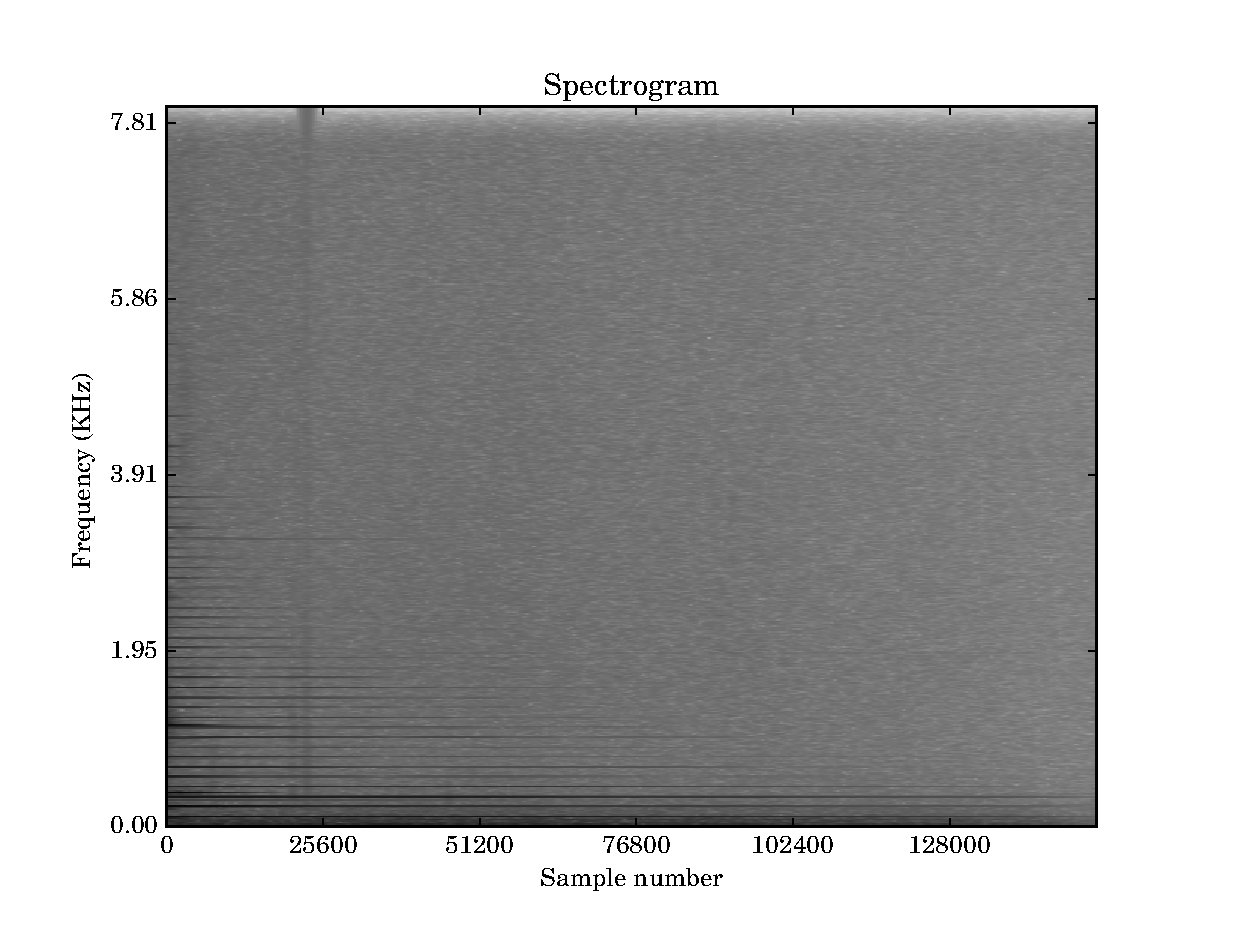
\includegraphics[width=\figwidthscale\textwidth]{plots/partial_estimation_acgtr_xylo_specgram.eps}
    \CaptionWithTitle{%
        \input{plots/partial_estimation_acgtr_xylo_specgram.txt}%
    }{\label{plot:acgtra3xylofs4specgram}}
\end{figure}

\begin{figure}[!t]
    \centering
    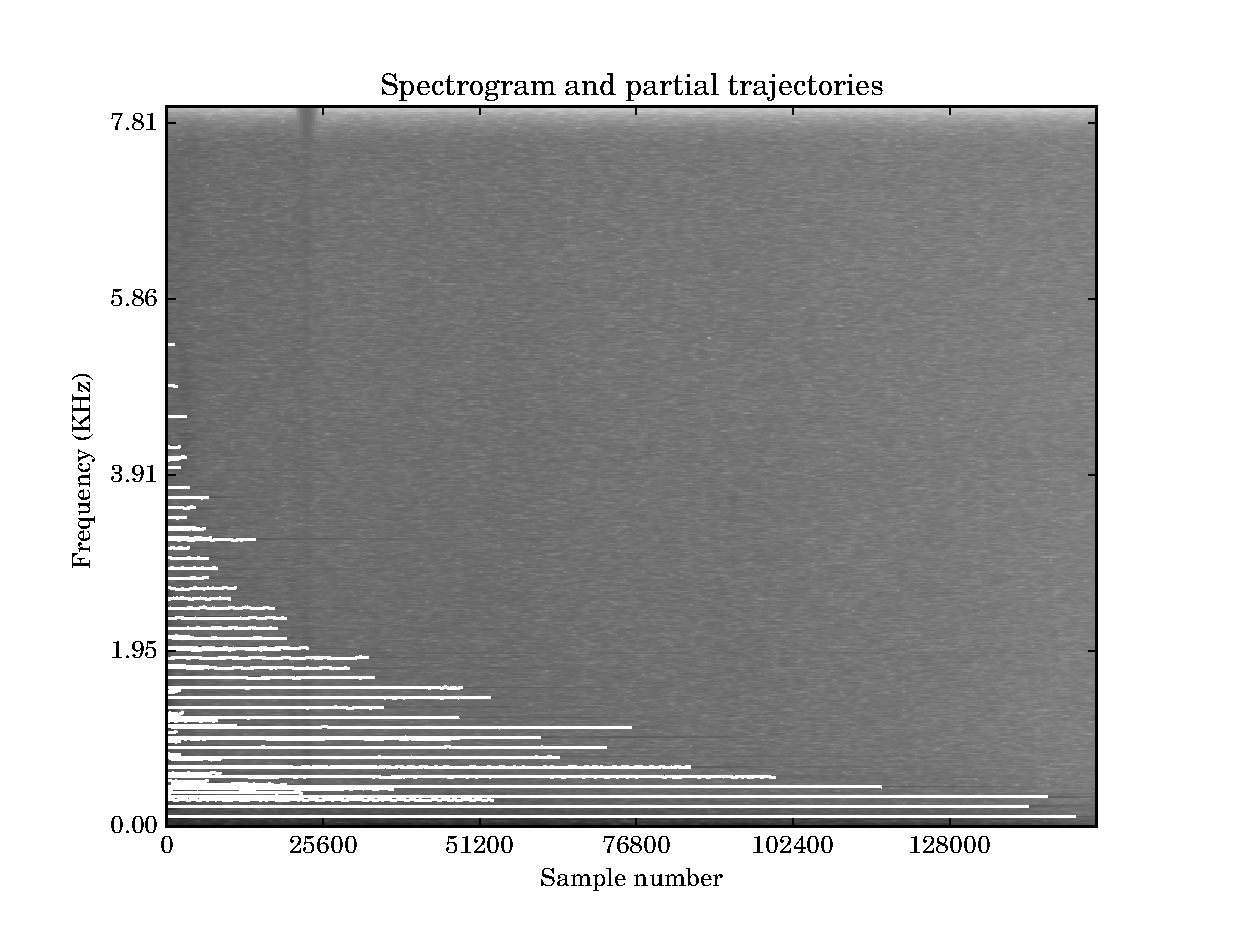
\includegraphics[width=\figwidthscale\textwidth]{plots/partial_estimation_acgtr_xylo_specgram_partials.eps}
    \CaptionWithTitle{%
        \input{plots/partial_estimation_acgtr_xylo_specgram_partials.txt}%
    }{\label{plot:acgtra3xylofs4partials}}
\end{figure}

\begin{figure}[!t]
    \centering
    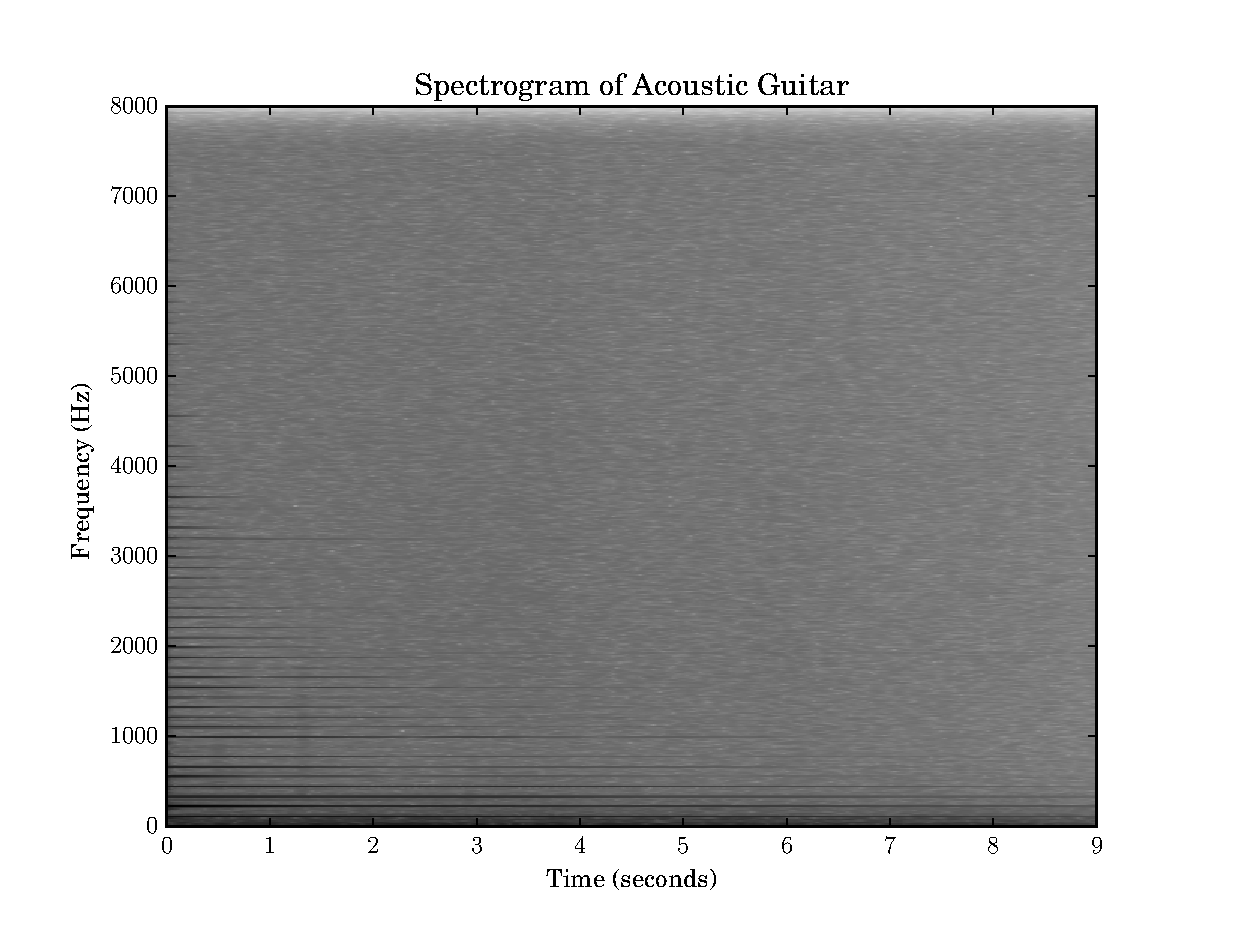
\includegraphics[width=\figwidthscale\textwidth]{plots/ac_gtr_orig_spec.eps}
    \CaptionWithTitle{%
        \input{plots/ac_gtr_orig_spec.txt}%
    }{\label{plot:acgtra3specgram}}
\end{figure}

\begin{figure}[!t]
    \centering
    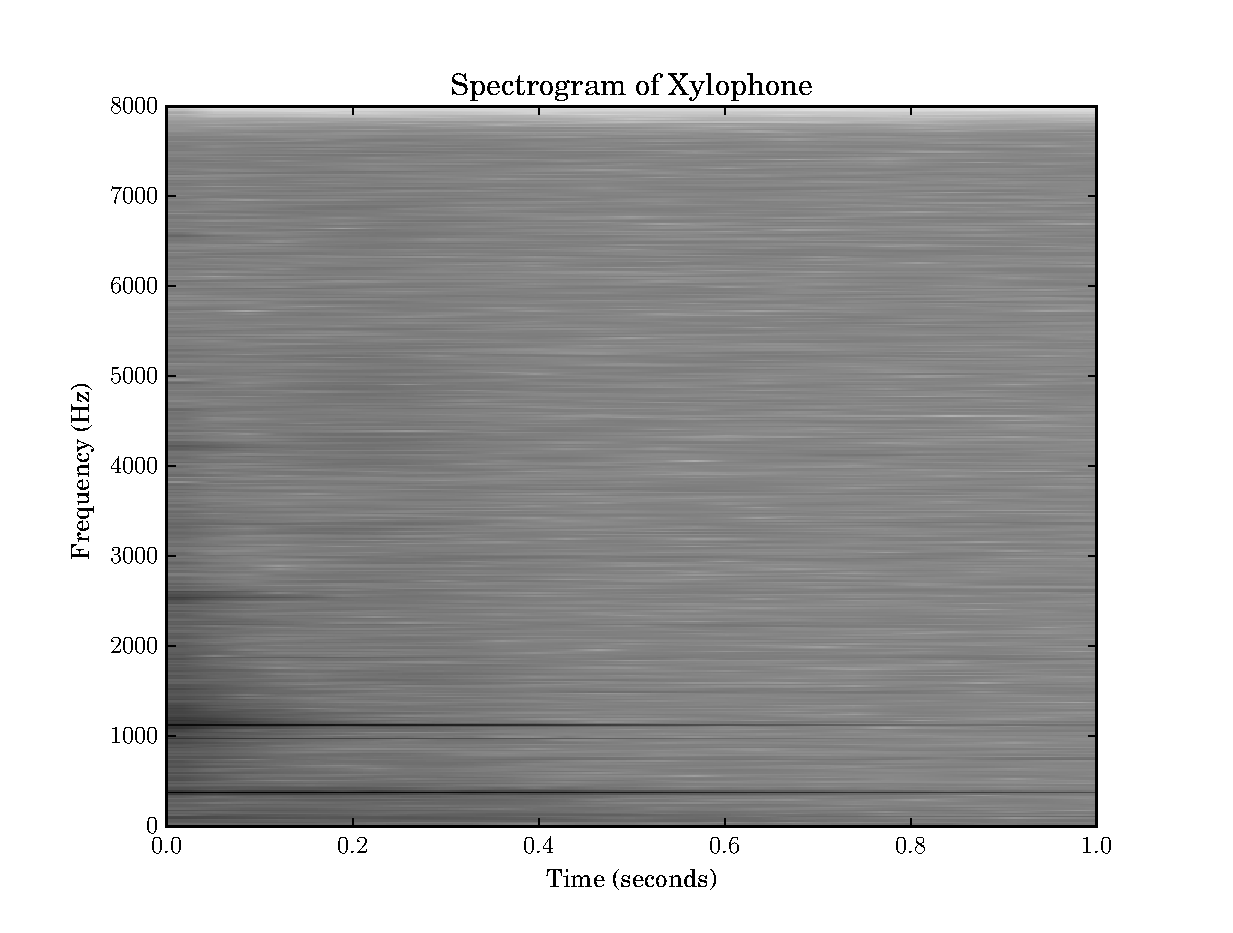
\includegraphics[width=\figwidthscale\textwidth]{plots/xylo_orig_spec.eps}
    \CaptionWithTitle{%
        \input{plots/xylo_orig_spec.txt}%
    }{\label{plot:xylofs4specgram}}
\end{figure}

\begin{figure}[!t]
    \centering
    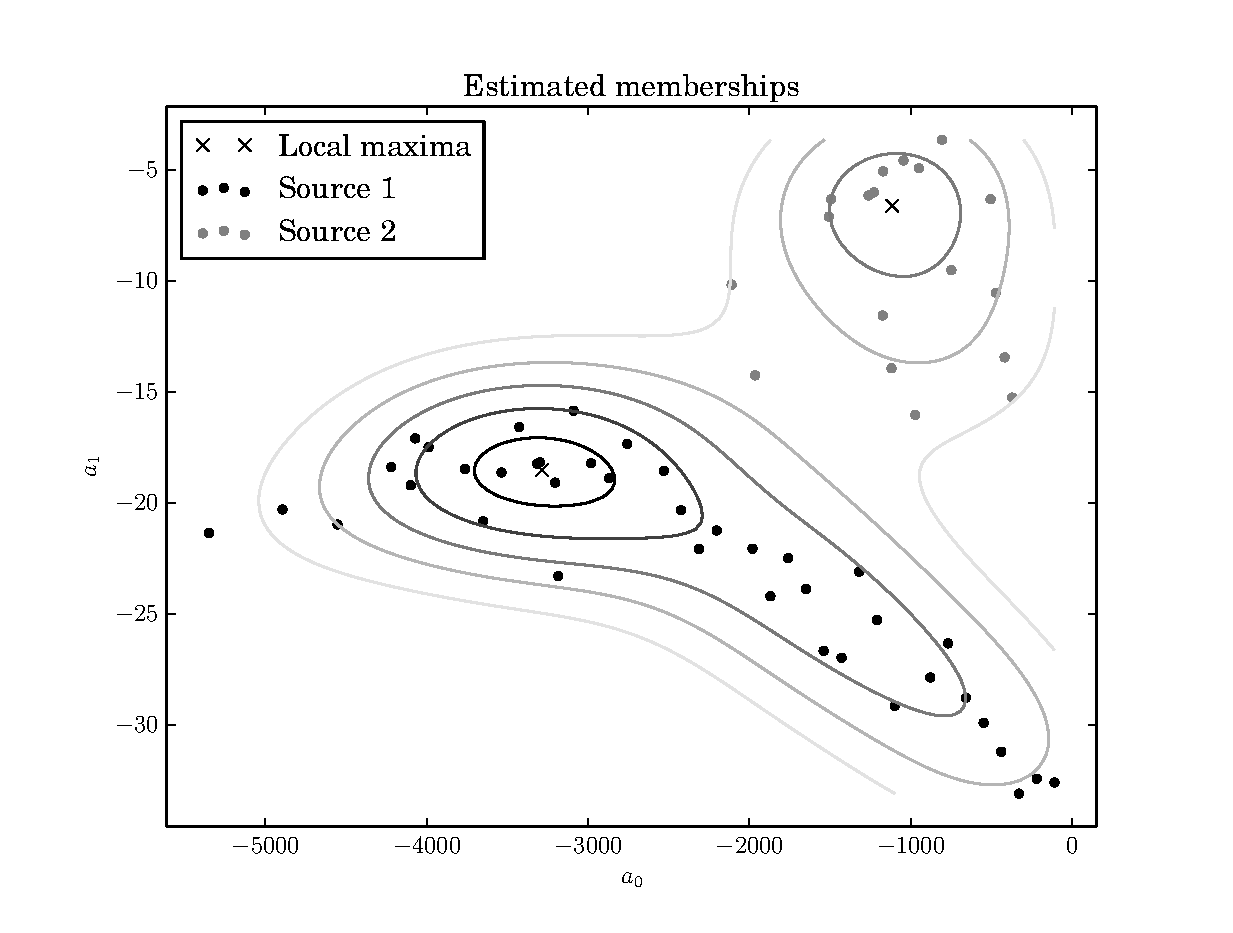
\includegraphics[width=\figwidthscale\textwidth]{plots/partial_classification_acgtr_xylo_estimated_memberships.eps}
    \CaptionWithTitle{%
        \input{plots/partial_classification_acgtr_xylo_estimated_memberships.txt}%
    }{\label{plot:partialclassificationacgtrxylosepestimatedmemberships}}
\end{figure}

\begin{figure}[!t]
    \centering
    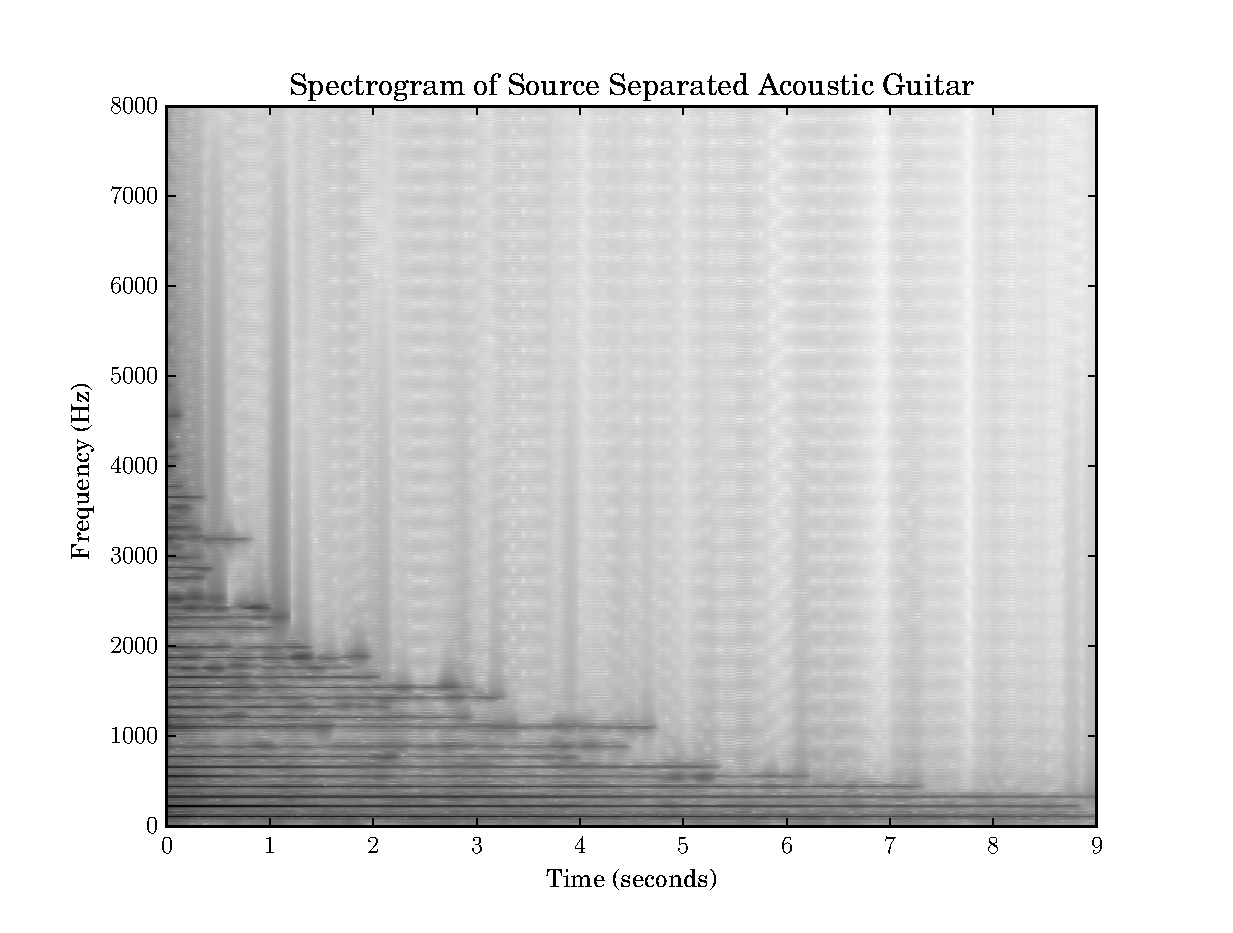
\includegraphics[width=\figwidthscale\textwidth]{plots/ac_gtr_ss_spec.eps}
    \CaptionWithTitle{%
        \input{plots/ac_gtr_ss_spec.txt}%
    }{\label{plot:acgtra3specgramss}}
\end{figure}

\begin{figure}[!t]
    \centering
    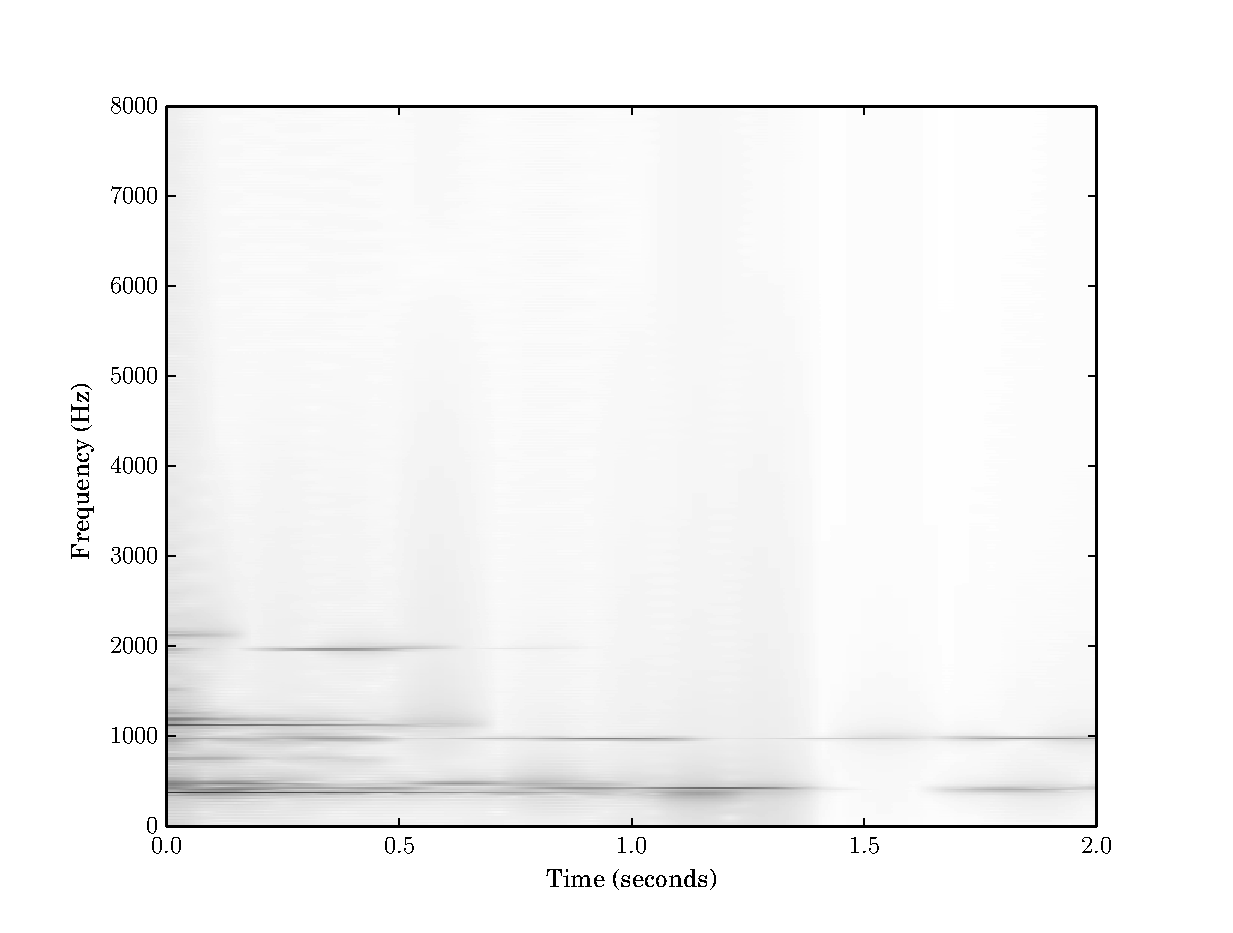
\includegraphics[width=\figwidthscale\textwidth]{plots/xylo_ss_spec.eps}
    \CaptionWithTitle{%
        \input{plots/xylo_ss_spec.txt}%
    }{\label{plot:xylofs4specgramss}}
\end{figure}

\section{Introduction}

In this section we demonstrate how the techniques described above can be used to
perform audio source separation on signals obtained from recordings of acoustic
instruments. Specifically, we show that in the absence of frequency-modulation,
amplitude modulation --- the decay rate --- can be used to classify partials
in a mixture of two sources into two groups, each group representing an
underlying source.

\section{Description of problem}

We start with a recording of an acoustic guitar playing $\text{A}_{3}$ and
a xylophone playing $\text{F}_{4}^{\sharp}$.  The recordings are from
\cite{opolko1987mcgill} and have been mixed down to one channel (by simply
adding the two signals together) and resampled at 16 kHz, coded simply as a
stream of 64-bit floating-point numbers. Spectrograms of the original signals
are shown in Figure~\ref{plot:acgtra3specgram} and
Figure~\ref{plot:xylofs4specgram}. The spectrograms were produced with a Hann
window, DFT size of 4096 samples and a hop size of 512 samples. We see that
neither source exhibits much frequency-modulation. The spectrogram of
the mixture can be seen in Figure~\ref{plot:acgtra3xylofs4specgram} and the
partial paths in Figure~\ref{plot:acgtra3xylofs4partials}.

The mixture of the two signals was analysed using the DDM for finding the
coefficients of a cubic complex phase polynomial. Local maxima in each frame
were found using the technique described in \cite[p.~42]{serra1989system}. For
each of these local maxima, the polynomial coefficients were estimated. The
analysis used the $\mathcal{C}^{1}$ 4-Term Blackman-Harris window that was
designed in Chapter~\ref{chap:sigmod}. To obtain
partials it was then necessary to connect the local maxima. As the partials of
these two sound sources are quite stable in frequency it sufficed to use the
Viterbi algorithm \cite{forney1973viterbi} and the cost metric
$\mathcal{D}_{\text{pr.}}$ from Section~\ref{sec:mq_lp_compare_chirp} to connect
local maxima in sub-bands of the spectrum. The cost function is simply the
Euclidean distance between the frequencies of two local maxima. Partial starting
points are considered in sub-bands of width 15 Hz and these sub-bands overlap by
7.5 Hz. A partial path starts on the first local maximum in the band exceeding
-100 dB and ends at the last maximum exceeding -100 dB. The path search
algorithm will also look ahead to further frames if no maximum is present in the
next frame. Because of this, sometimes unrealistic paths are discovered that
jump between spurious maxima. These are filtered out by discarding paths whose
cost-length ratio is excessive. See
Figure~\ref{plot:acgtra3xylofs4costlengththresh} to see a plot of these values
and the thresholding function. 

\section{Motivation}

A line function is fit via least-squares to each partial, as shown in
Figure~\ref{plot:parclassaxpartialtrajectories}. Our goal is to classify based
on the amplitude modulation of each partial, or to an approximation, the slope of these line functions. We found that examining the log-length of the
partials gives better results than examining the slope directly. This is perhaps
because the log-length encodes both the starting amplitude and the slope. Recall
that the partials start on the first local maximum exceeding an amplitude
threshold --- those with lower starting amplitude and steeper amplitude slope will be
shorter, while those with a higher starting amplitude and shallower slope will
be longer. We see in
Figure~\ref{plot:partialclassificationacgtrxyloseptruememberships} that using
both the amplitude-slope and the initial amplitude of the partial gives clear
separation in a plot of the log-length vs.\ the
average frequency of
the partials. These partials are from separate overlaid analyses of the guitar
and xylophone signals. The experiment uses an analysis of a signal consisting of
a mixture of the sources, of course.

The data-points have the form
\[
    \boldsymbol{a}_i = \begin{pmatrix}
        a_{i,0} \\
        a_{i,1}
    \end{pmatrix}
\]
where $a_{i,0}$ is the first principal components and $a_{i,1}$ the second and are computed via a
linear transformation of
\[
    \boldsymbol{x}_i
    =
    \begin{pmatrix}
        \overline{f}_{i} \\
        \ell_{i}
    \end{pmatrix}
\]
where $\overline{f}_{i}$ is the mean frequency of the $i$th partial and
$\ell_{i}$ its log-length (see
Appendix~\ref{chap:pca} for the computation of principal components). The set of
principal components will be denoted $\{\boldsymbol{a}\}$.
We see that, for the most part, the partials belonging to the two sources are
separated appropriately into two clusters. The partials from the xylophone
present in the guitar cluster belong to higher partials, whose omission in the
final rendering of the xylophone source would not be detrimental to its
perceptual quality. Similarly, partials belonging to the guitar present in the
xylophone cluster are short and most likely belong to briefly excited modes
of the guitar body.

\section{Classification}

Our intention is now to use GMM on a set of unclassified partials to yield a
plausible source separation. GMM fitting is sensitive to its initial guess of
the parameters as the algorithm can converge to a local maximum of the likelihood
function \cite[p.~187]{kay1993fundamentals}.  To find an initial guess we
convolve the scatter plot with kernel $\mathscr{K}$, giving a continuous function.
$\mathscr{K}$ is defined%
\footnote{Note its similarity to the normal distribution, defined in
Appendix~\ref{chap:normaldist}.}
\[
    \mathscr{K}(\boldsymbol{x},\boldsymbol{\beta})
    =
    \exp(\D-\frac{1}{2}\boldsymbol{x}^{T}\boldsymbol{\beta}^{-1}\boldsymbol{x})
\]
Here $\boldsymbol{x} \in \mathbb{R}^{2}$ and $\boldsymbol{\beta} \in
\mathbb{R}^{2 \times 2}$ controls the extent of the kernel, i.e., how much it
smooths in each dimension. 

We use the two local maxima of this function as the initial means for the two
sought classifying Gaussian distributions. The convolution function evaluated
at $\boldsymbol{\hat{a}}$ is
\[
    f(\boldsymbol{\hat{a}}) = \sum_{\boldsymbol{a}_i \in \{\boldsymbol{a}\}}
    \mathscr{K} \left( \boldsymbol{\hat{a}} - \boldsymbol{a}_i,
    \boldsymbol{\beta}_{\boldsymbol{a}} \right)
\]
To make the variance proportional to the extent of each dimension,
$\boldsymbol{\beta}_{\boldsymbol{a}}$ is defined as
\[
    \boldsymbol{\beta}_{\boldsymbol{a}}
    =
    \begin{pmatrix}
        \frac{\D\Delta_{\boldsymbol{a}_1}}{\D\Delta_{\boldsymbol{a}_0
        +\Delta_{\boldsymbol{a}_1}}}
            \theta_{\boldsymbol{\beta}_{\boldsymbol{a}}}
        & 0 \\
        0 & \frac{\D\Delta_{\boldsymbol{a}_0}}{\D\Delta_{\boldsymbol{a}_0
    +\Delta_{\boldsymbol{a}_1}}}
            \theta_{\boldsymbol{\beta}_{\boldsymbol{a}}}
    \end{pmatrix}
\]
where
\[
    \Delta_{\boldsymbol{a}_0} = \max \left( \boldsymbol{a}_0 \right)
        - \min \left( \boldsymbol{a}_0 \right)
\]
\[
    \Delta_{\boldsymbol{a}_1} = \max \left( \boldsymbol{a}_1 \right)
        - \min \left( \boldsymbol{a}_1 \right)
\]
and $\theta_{\boldsymbol{\beta}_{\boldsymbol{a}}}$ is a parameter to control
the smoothness of the resulting function, here
$\theta_{\boldsymbol{\beta}_{\boldsymbol{a}}} = 1.2$. A contour plot of the
resulting function $f(\boldsymbol{\hat{a}})$ is shown in
Figure~\ref{plot:partialclassificationacgtrxylosepestimatedmemberships}.

To initialize GMM the initial means $\boldsymbol{\mu}^{0}$ are chosen to be the
points corresponding to the local maxima of the smoothed scatter plot%
\footnote{Recall that the superscript here refers to the iteration number of the
algorithm.}. To
determine initial weights $\boldsymbol{w}^{0}$ we first determine the value of
the function at the two local maxima, $f(\boldsymbol{a}_{0}^{\ast})$ and
$f(\boldsymbol{a}_{1}^{\ast})$. To weight relative to these two values, we
compute
\[
    w_{i}^{0} = \frac{\Theta_{w} \left\{ f(\boldsymbol{a}_{i}^{\ast}) \right\}}{
    \sum_{p=0}^{R-1}\Theta_{w} \left\{ f(\boldsymbol{a}_{p}^{\ast} \right\}}
\]
where $\Theta_{w}$ is some kind of weighting operator to have parametric control
over the influence of each function value and $R$ is the number of maxima. Here
\[
    \Theta_{w} \left\{ f(\boldsymbol{a}_{i}^{\ast}) \right\}
    = \begin{cases}
        f(\boldsymbol{a}_{i}^{\ast}) \theta_{w} & i = 0 \\
        f(\boldsymbol{a}_{i}^{\ast}) & \text{otherwise}
    \end{cases}
\]
and $R = 2$, i.e., only the first maximum is weighted. For this experiment the parameter set as $\theta_{w} = 1.1$ gave
the best results. The covariance matrix $\boldsymbol{\Sigma}^{0}$ is computed as
\[
    \boldsymbol{\Sigma}^{0} = \boldsymbol{S}(\{ \boldsymbol{a} \}) +
    \epsilon\boldsymbol{I}
\]
where $\boldsymbol{S}$ computes the sample covariance and
$\boldsymbol{\epsilon}\boldsymbol{I}$ is a matrix whose only non-zero entries
are on the main diagonal and are equal to a small constant to avoid a singular
initial covariance matrix. 100 iterations of the EM algorithm are performed to
compute classifications. Each point is assigned to its most likely cluster using
the final estimated Gaussian distributions. The final classifications for this
classification task can be seen in
Figure~\ref{plot:partialclassificationacgtrxylosepestimatedmemberships}.

\section{Synthesis}

After the classifications have been made, synthesizing the separated sources
simply involves only synthesizing the partials classified as belonging to the
same source. For the synthesis, we use the technique described in
Section~\ref{sec:s23synthesis}. Spectrograms of the source separated signals
are shown in Figure~\ref{plot:acgtra3specgramss} and
Figure~\ref{plot:xylofs4specgramss}. 

\section{Conclusion}

After an informal listening, the source separation is perceptually
convincing.\footnote{Soundfiles can be downloaded from \par
\url{https://drive.google.com/file/d/0B8B4c04j8tBwZDFraEZ1dFZHRFU/view?usp=sharing}}
At least one partial from the guitar can be heard in the xylophone recording,
however --- it is difficult to separate partials that do not have sufficient
spacial separation in
Figure~\ref{plot:partialclassificationacgtrxylosepestimatedmemberships}. Another
drawback of the current technique is that it requires some tuning of the
parameters $\theta_{w}$ and $\theta_{\boldsymbol{\beta}_{\boldsymbol{a}}}$.
From the spectrograms of the resynthesized sources, we see that some of the
partials from both sounds were lost in the analysis.  Although a shortcoming of
the analysis rather than the classification, if partials are not sufficiently
separated in time or frequency, they cannot be separated as their analysis will
yield simply one partial when there are in fact many. In any case, it is important
to see that source separation can be carried out by only considering the
amplitude modulation (in this case, the decay rate) in relation to the partial
frequency.
